\section{双机异步通信中断发送,查询接收实现}
双机通过中断发送,查询接收实现实现互相通信,并增加小灯以作展示。
\subsection{原理分析}
在异步通信中断发送实现的基础上,加入双机异步通信查询接收\\
\\
原理图如下:\\
\begin{figure}[htbp]
  \centering
  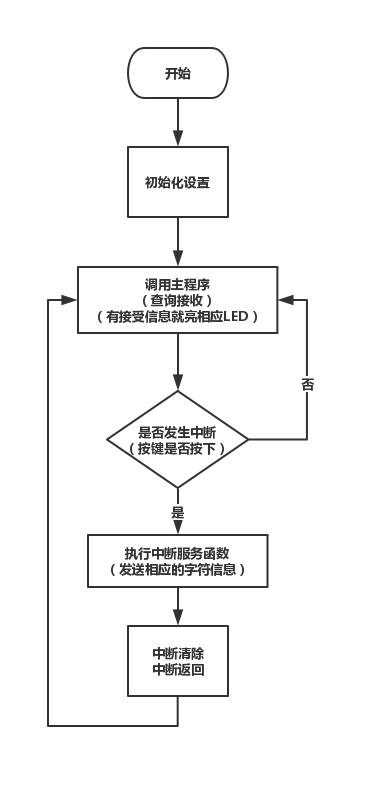
\includegraphics[width=0.3\textwidth]{sch4.png}
  \caption{双机异步通信中断发送,查询接收实现原理图}
\end{figure}
\\
\subsection{调试过程}
\subsubsection{主程序}
\lstset{language=C}
\begin{lstlisting}{主程序}
    int main()
    {
        unsigned char c;
        uart0_init();  
        GPFCON &= ~(GPF4_msk | GPF5_msk | GPF6_msk);
        GPFCON |= GPF4_out | GPF5_out | GPF6_out;
    
        while(1)
        {
            c = getc();
            if (c == 'a'){
                GPFDAT &= ~(1<<4);
                GPFDAT |= (1<<5);
                GPFDAT |= (1<<6);
            } 
            else if (c == 'b'){
                GPFDAT |= (1<<4);
                GPFDAT &= ~(1<<5);
                GPFDAT |= (1<<6);
            }
            else if (c == 'c'){
                GPFDAT |= (1<<4);
                GPFDAT |= (1<<5);
                GPFDAT &= ~(1<<6);
            }
        }
        return 0;
    }
\end{lstlisting}
没有按下按键时,其一直在查询uart0寄存器的数值,若有接收,则点亮对应的灯。
当按下对应按键的时候,uart0会发送出"a","b","c"等字母。


\subsection{结果}
当按下对应按键的时候,对方机子会亮对应的灯,反之亦是。
\begin{figure}[htbp]
    \centering
    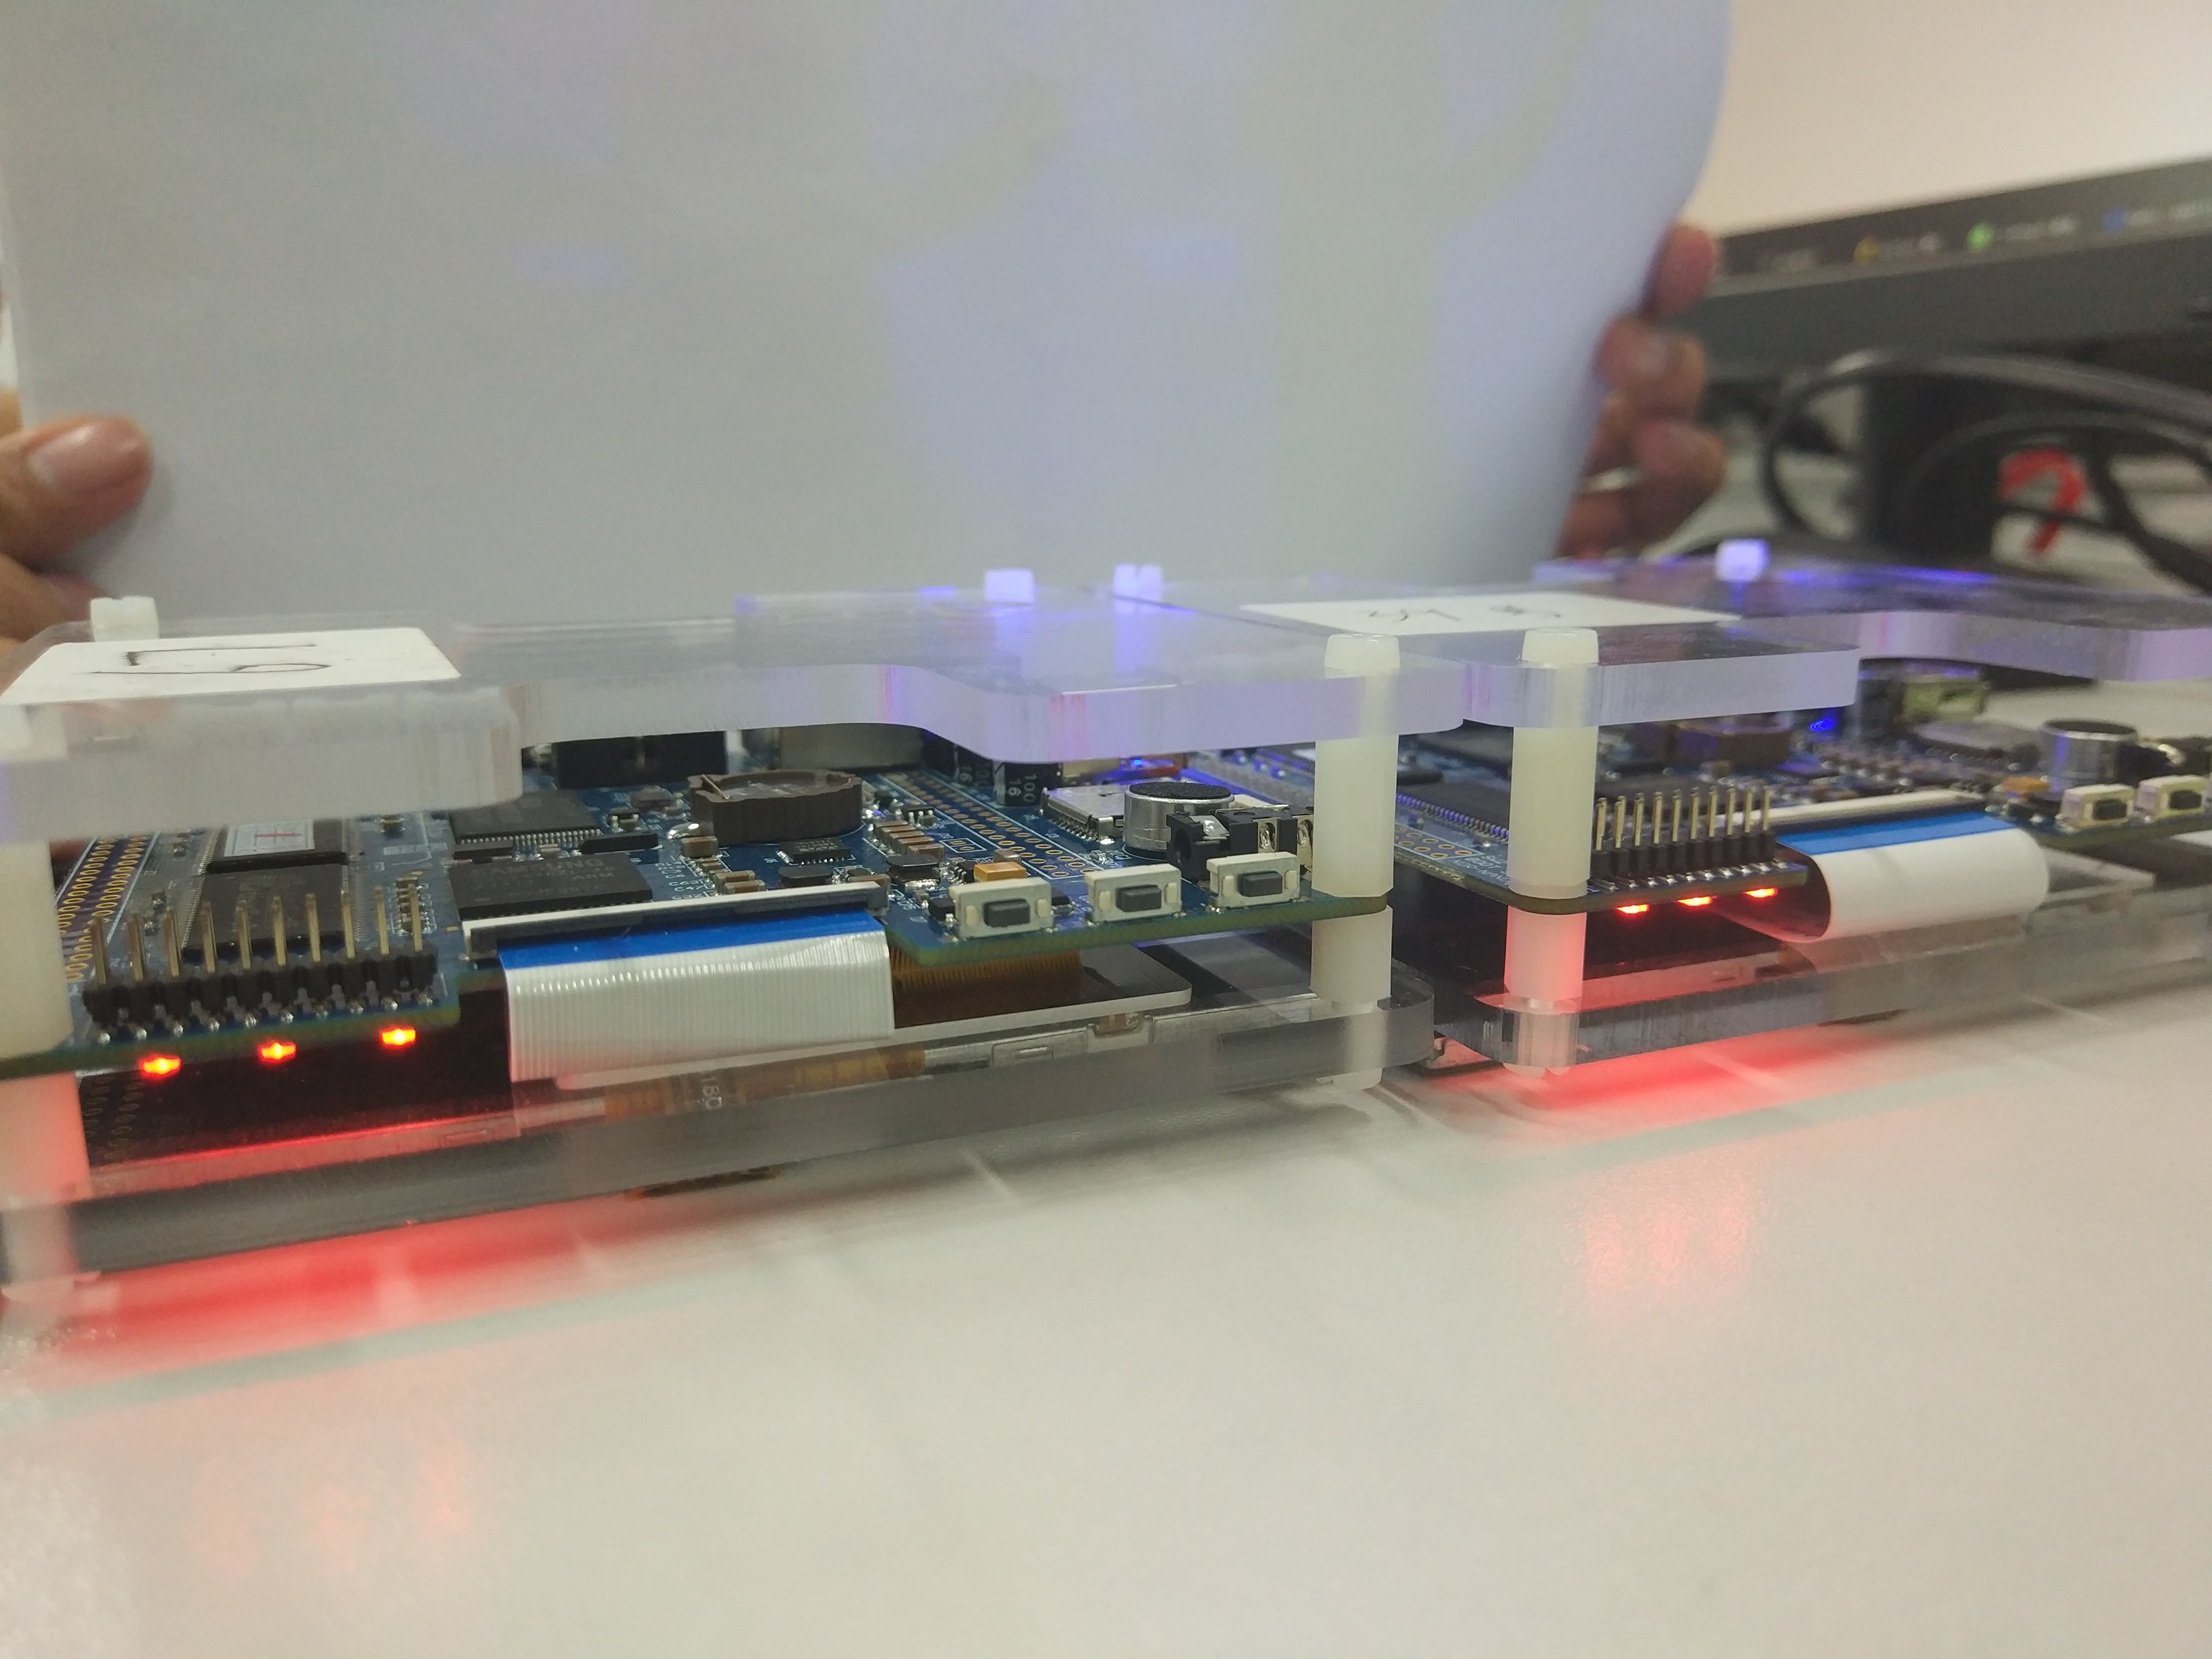
\includegraphics[width=0.5\textwidth]{result4-1}
    \caption{原始状态}
\end{figure}

\begin{figure}[htbp]
    \centering
    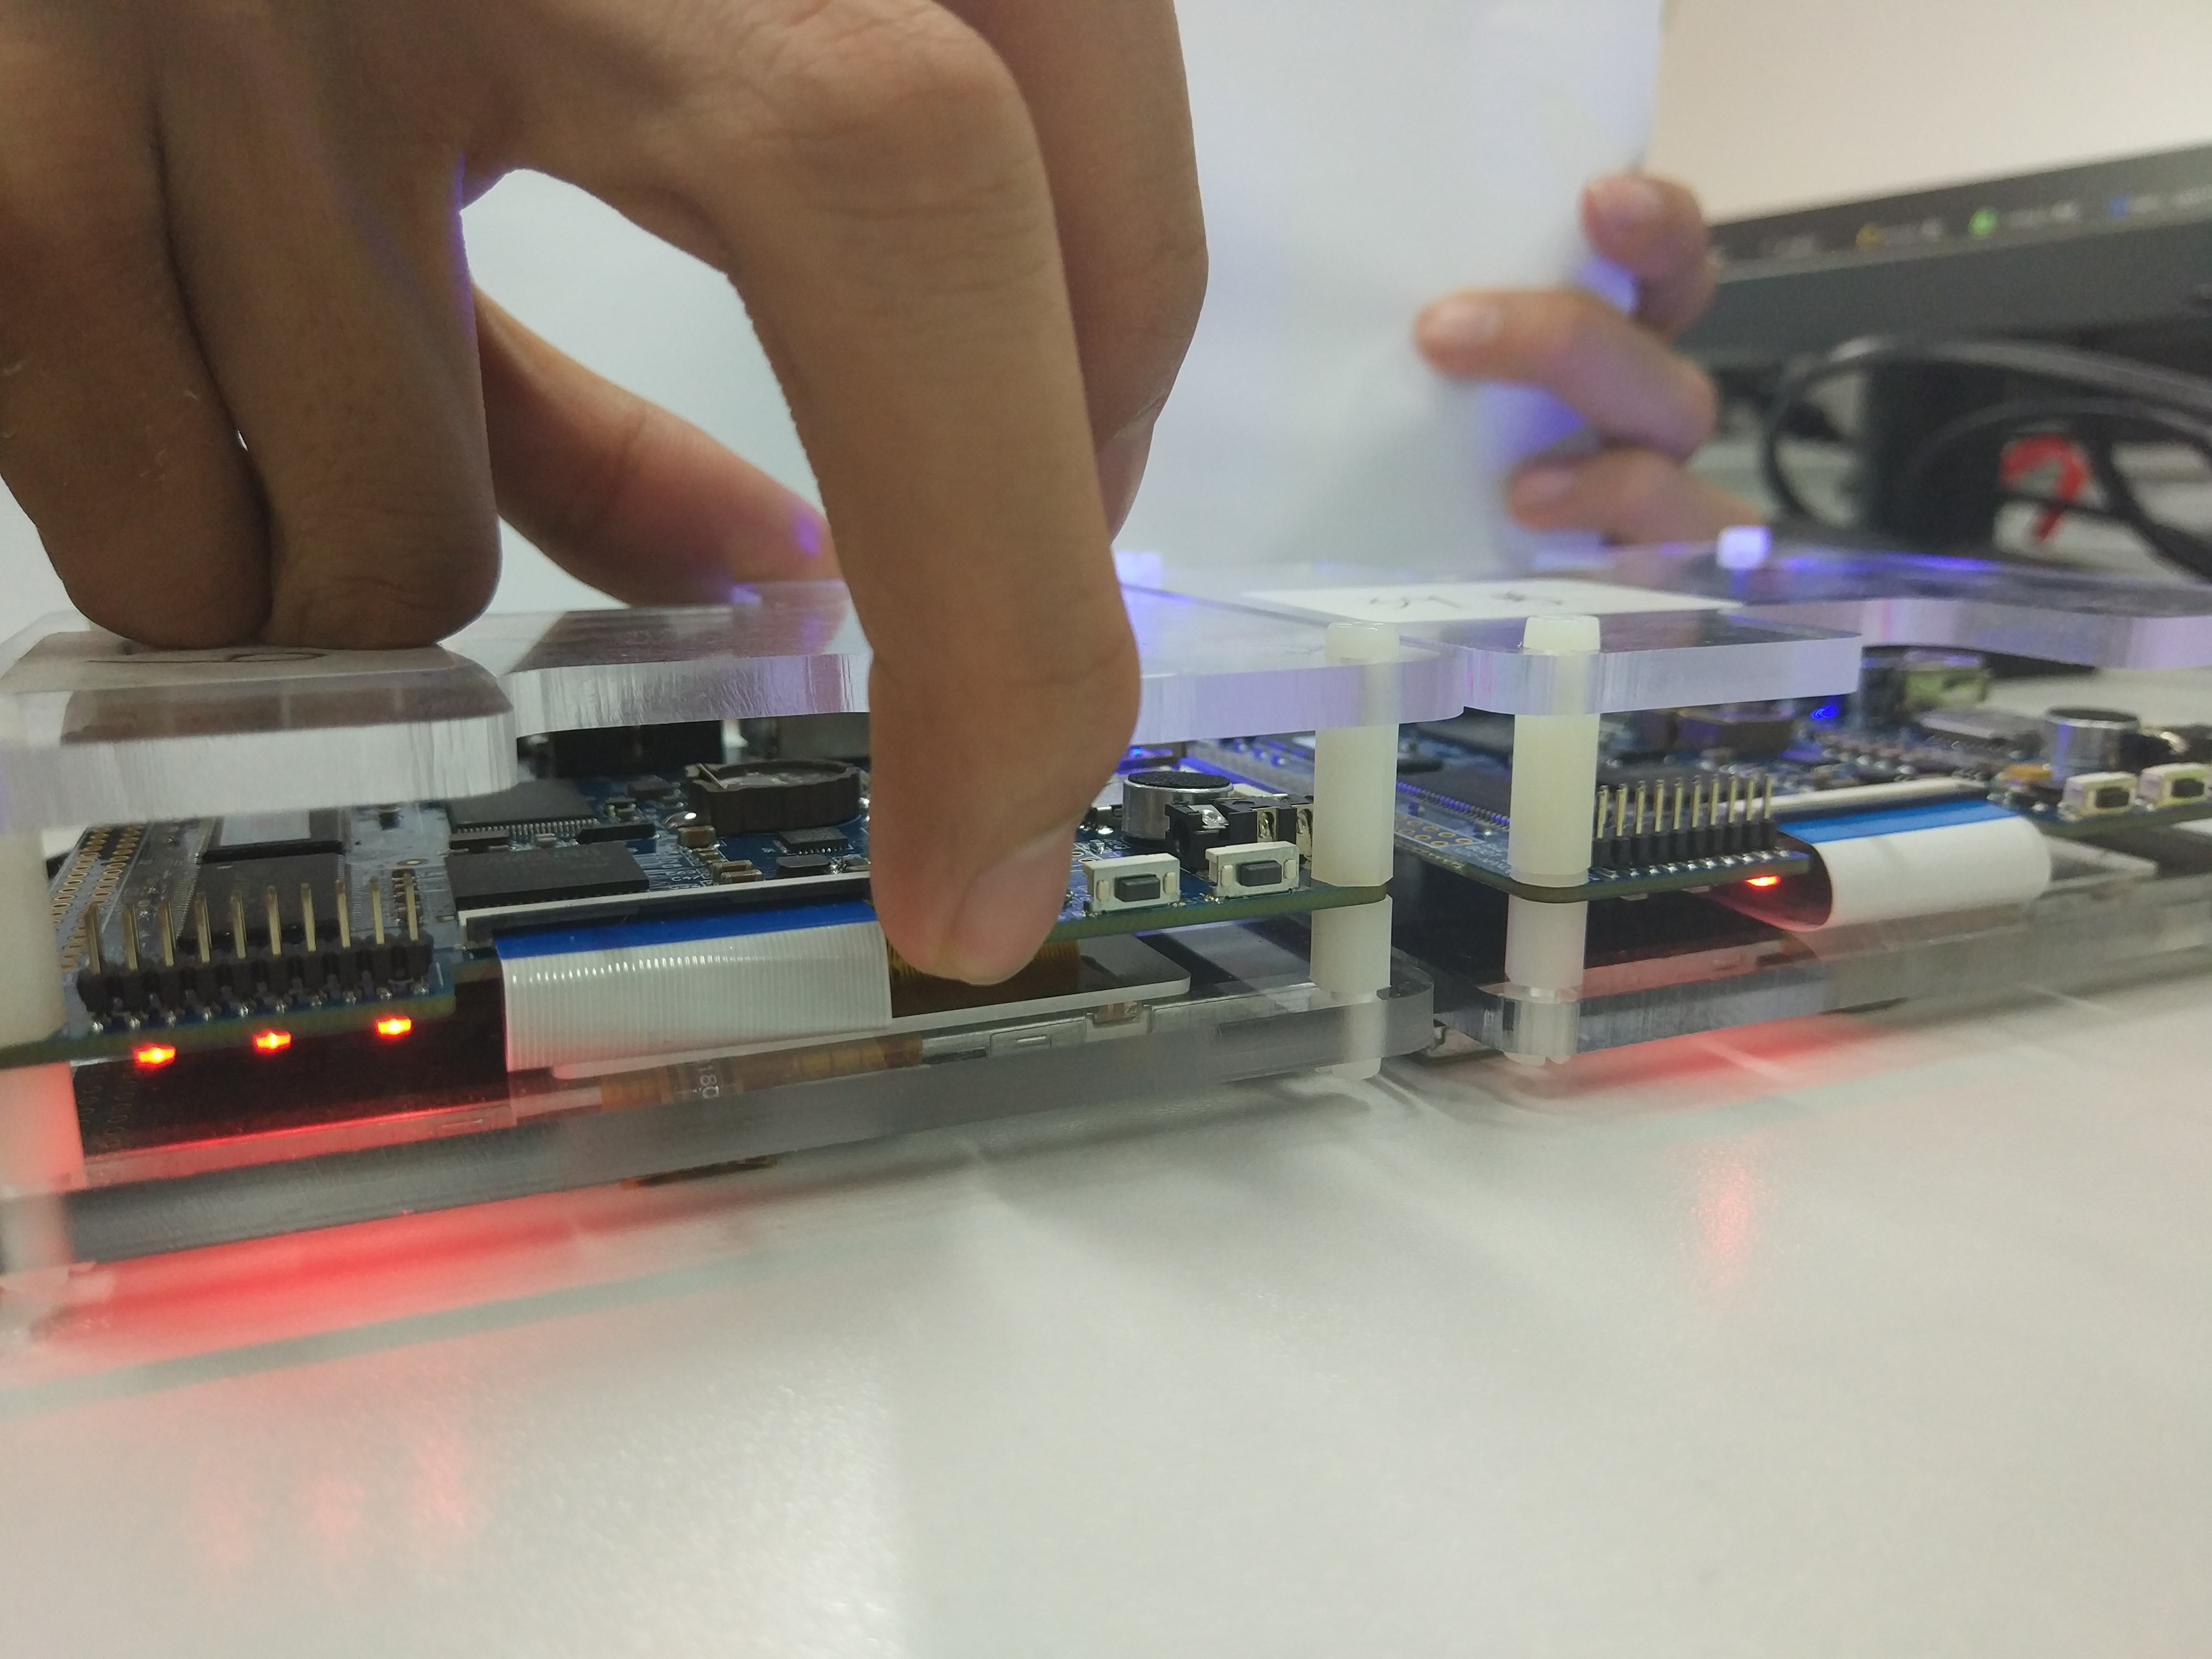
\includegraphics[width=0.5\textwidth]{result4-2}
    \caption{按下1号机子}
\end{figure}

\begin{figure}[htbp]
    \centering
    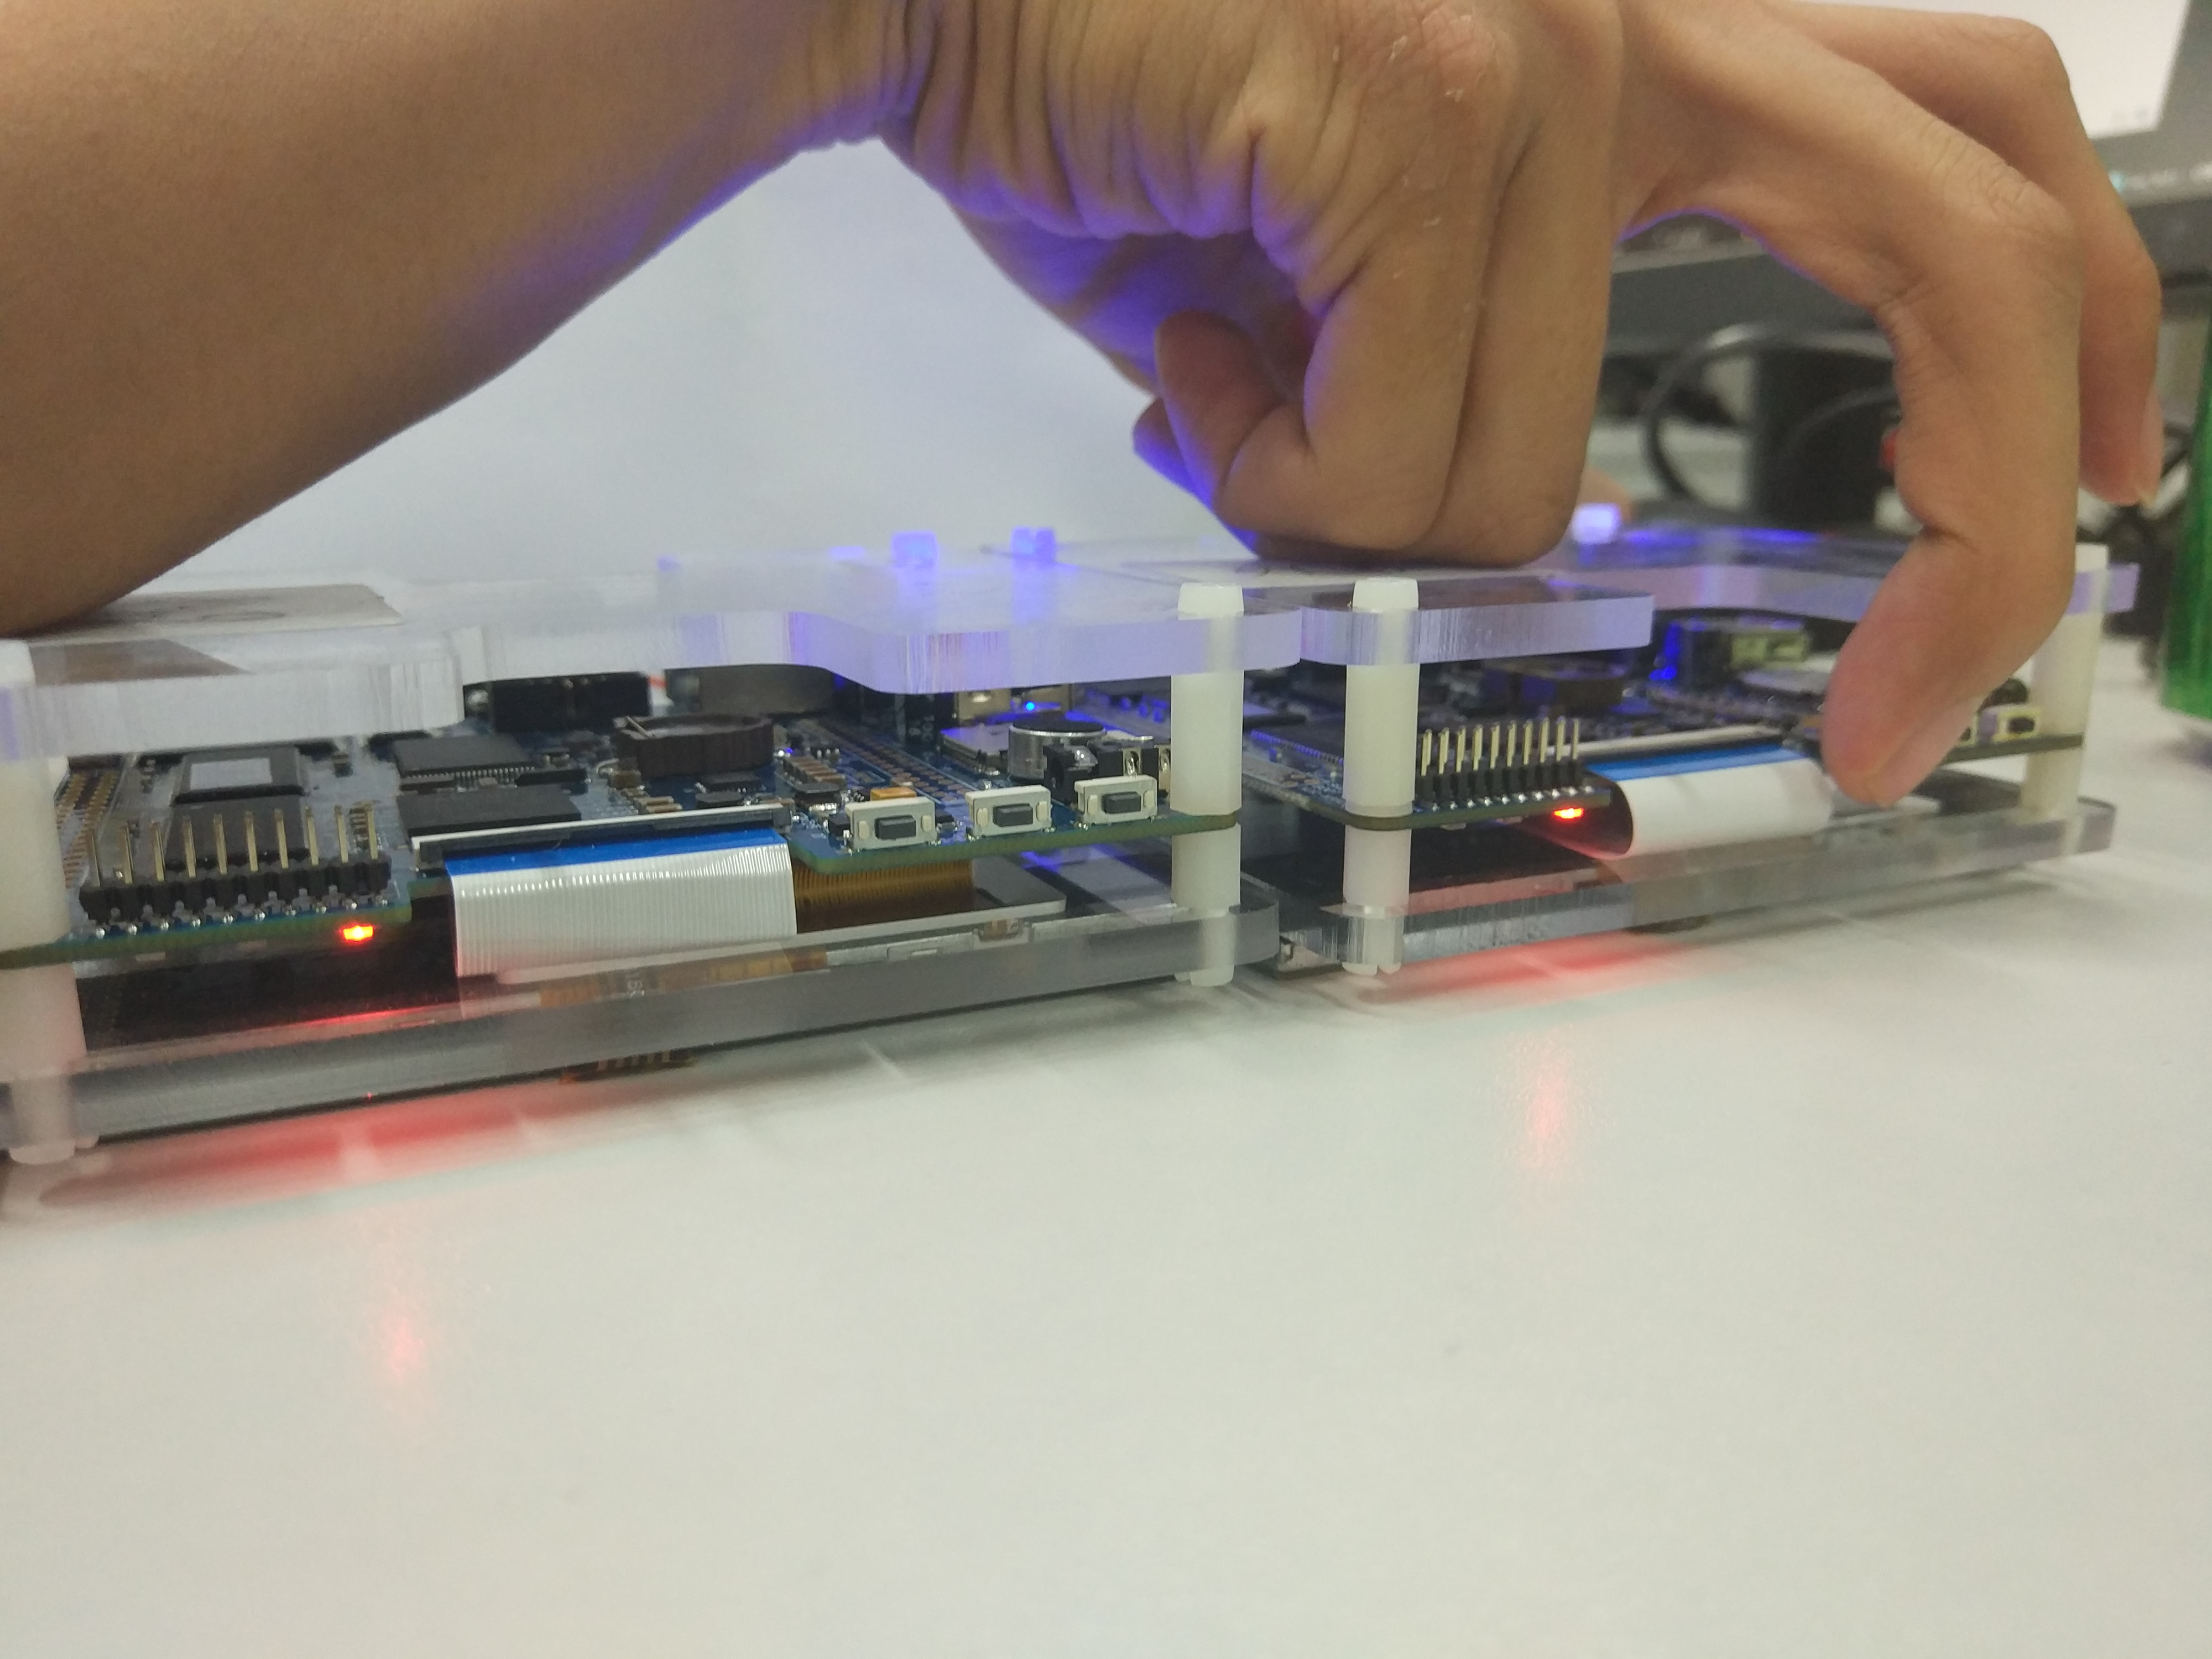
\includegraphics[width=0.5\textwidth]{result4-3}
    \caption{按下2号机子}
\end{figure}
\subsection{问题与总结}
使用的是查询接收,效率不高,需进一步改进。